\section{Design Specification}
Our crisis mapping system was written in two different programming languages, Python and Javascript. We had to choose Python because the Gaussian Process library was implemented in this language. We chose JavaScript simply because it is easier to do pretty user-interface programming and we had working experience with it. Figure \ref{fig:system-overview} shows an overview of the system.

\begin{figure}[here]
  \centering
      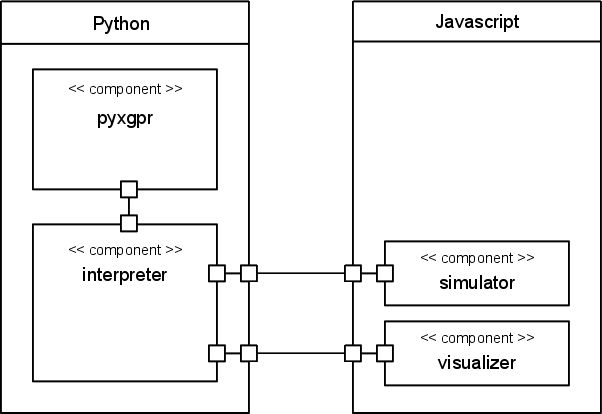
\includegraphics[width=0.7\textwidth]{solution/graphics/system-overview.png}
  \caption{System overview.}
  \label{fig:system-overview}
\end{figure}

The system is not large and there is one main flow in the system. A fire situation is simulated and sampled in the simulator. The samples are sent to the interpreter. The interpreter will try to reconstruct the fire situation and send the result back to the visualizer to view the result. The actual fire situation and the reconstructed are then available for comparison in the Javascript system.